\chapter{Teorema de Fubini}
	\section{Teorema de Fubini}
	
	\begin{teor} Teorema de Fubini para $\R^2$.\\
	Sea $\function{f}{[a,b]\times[c,d]}{\R}$ integrable.\\
	Supongamos que $\forall x\in [a,b]$ la función $\xfunction{f_x}{[c,d]}{\R}{y\to f(x,y)}$ es integrable en $[c,d]$, entonces la función $\xfunction{\varphi}{[a,b]}{\R}{x\to\integral{d}{c} f_x=\integral{d}{c} f(x,y)dy}$ es integrable y $\integral{}{[a,b]\times[c,d]} f=\integral{b}{a}\left(\integral{d}{c}f(x,y)dy\right)dx$
	\end{teor}
	
	\begin{proof}\ \\
Definamos la función $\xfunction{f_x}{[c,d]}{\R}{y\to f(x,y)}\ \forall x\in[a,b]$, tenemos que $f_fgx$ es integrable. Podemos definir ahora $\function{F}{[a,b]}{\R}\talque F(x)=\integral{d}{c}f_x=\integral{d}{c}f(x,y)dy$.\\
Probemos que $F$ es integrable y que $\integral{b}{a}F=\integral{}{[a,b]\times[c,d]}f$.\\
Supongamos que se cumple la hipótesis. Sea $\varepsilon>0,\ \exists p=(p_1,p_2)\in\pi([a,b]\times[c,d])$ tal que $p_1=\{a=t_0,t_1,...,t_n=b\}$ (con $[t_{i-1},t_i]=I_i$) y $p_2\{c=s_0,s_1,...,s_m=d\}$ (con $[S_{j-1},s_j]=\\=J_j$).
Tenemos $\integral{}{[a,b]\times[c,d]}f-\varepsilon\leq s(f,p)=\stackbin[i=1]{n}\sum\left(\stackbin[j=1]{m}\sum\inf\{f(x,y)\talque x\in I_i,\ y\in J_j\}\cdot v(I_i)\right)v(J_j)$\\
Fijemos $i_0\y x_0\in I_{i_0}$, tenemos:\\
$\stackbin[j=1]{m}\sum\inf\{f(x,y)\talque x\in I_0,\ y\in J_j\}v(J_j)\leq\stackbin[j=1]{m}\sum\in\{f(x_0,y)\talque y\in J_j\}v(J_j)=s(f_{x_0}(y),p_2)\implies$\\
$\implies s(f_{x_0}(y),p_2)\leq\integral{d}{c}f_{x_0}=F(x_0)$.\\
Por lo tanto tenemos que $\stackbin[j=1]{m}\sum\inf\{f(x,y)\talque x\in I_{i_0},\ y\in J_j\}v(J_j)\leq F(t)\ \forall t\in I_{i_0}\implies\\
\implies\stackbin[j=1]{m}\sum\inf\{f(x,y)\talque x\in I_{i_0},\ y\in J_j\}v(J_j)\leq\inf\{F(t)\talque t\in I_{i_0}\}$, por tanto,\\
$\left(\stackbin[j=1]{m}\sum\inf\{f(x,y)\talque x\in I_i,\ y\in J_j\}v(J_j)\right)v(I_i)\leq\inf\{F(t)\talque t\in I_i\}v(I_i)\ \forall i\in\{1,..,n\}$\\.
Volviendo a la primera desigualdad,
$\stackbin[i=1]{n}\sum\left(\stackbin[j=1]{m}\sum\inf\{f(x,y)\talque x\in I_i,\ y\in J_j\}v(J_j)\right)v(I_i)\leq\\
\leq\stackbin[i=1]{n}\sum\inf\{F(x)\talque x\in I_i\}v(I_i)=s(F,p_1)\leq S(F,p_1)\leq\integral{}{}f+\varepsilon$.
\end{proof}
	
	\begin{teor} Teorema de Fubini generalizado para $\R^{n+m}$.\\
	Sean $R_1$, $R_2$ rectángulos, $R_1\subset \R^n, R_2\subset \R^m$ y sea $R=R_1\times R_2 \subset\R^{n+m}$. Sea $\function{f}{R}{\R}$ integrable, supongamos que $\forall x\in R_1$ la función $\xfunction{f_x}{R_2}{\R}{y\to f(x,y)}$ es integrable en $R_2$, entonces $\xfunction{\varphi}{R_1}{\R}{x\to\integral{}{R_2} f_x=\integral{}{R_2} f(x,y)dy}$ es integrable en $\R$ y $\integral{}{R} f=\integral{}{R_1}\left(\integral{}{R_2}f(x,y)dy\right)dx$
	\end{teor}
	
	\begin{observacion} Podemos intercambiar el papel de las variables.
	\end{observacion}
	
	\begin{ejem} \ 
	\begin{figura}\ 
	\begin{center}
	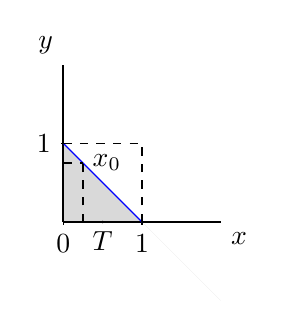
\begin{tikzpicture}
	\fill[color=gray!30]
(0,0) -- (0,1)
-- plot [domain=1:2] (\x,-\x+1)
-- (1,0) -- cycle;
		\draw[thick] (0,0) -- (2,0) node[anchor=north west] {$x$};
		\draw[thick] (0,0) -- (0,2) node[anchor=south east] {$y$};
		\foreach \x in {0,1}
   \draw (\x cm,1pt) -- (\x cm,-1pt) node[anchor=north] {$\x$};
    \foreach \y in {1}
    \draw (1pt,\y cm) -- (-1pt,\y cm) node[anchor=east] {$\y$};
		\draw [blue](0,1) -- (1,0);
		\draw [dashed](0,1) -- (1,1);
		\draw [dashed](1,0) -- (1,1);
		\draw [dashed](0.25,0) -- (0.25,0.75) node[anchor=west] {$x_0$};
		\draw [dashed](0,0.75) -- (0.25,0.75);
		\fill (0.5,0) circle (0.5pt)node[anchor=north] {$T$};
	\end{tikzpicture}
	\end{center}
	\end{figura}
	Calcular la integral de $\xfunction{f}{T}{\R}{(x,y)\to x}$\\\\
	
	$\integral{}{T}xdxdy=\integral{}{T}f(x,y)dxdy=\integral{}{[0,1]\times[0,1]}\overline{f}(x,y)dxdy\overset{\mathrm{Fubini}}= \integral{1}{0}\left(\integral{1}{0}\overline{f}(x,y)dy\right)dx$\\
	Tenemos:\\
	$\integral{1}{0}\overline{f}_{x_0}=\integral{1-x_0}{0}\underset{f(x_0,y)}{\underset{\shortparallel}{\overline{f}_{x_0}}}  + \integral{1}{1-x_0}\underset{0}{\underset{\shortparallel}{\overline{f}_{x_0}}}=\integral{1-x_0}{0}f(x_0,y)dy\implies \integral{}{T}f(x,y)dxdy=\\
	=\integral{1}{0}\left(\integral{1-x}{0}f(x,y)dy\right)dx=\integral{1}{0}\left(\integral{1-x}{0}xdy\right)dx=\integral{1}{0}x(1-x)dx=\left.\dfrac{x^2}{2}-\dfrac{x^3}{3}\right]^1_0=\dfrac{1}{6}$
	\end{ejem}
	\ \\
	\begin{ejem} \ 
	\begin{figura}\ 
	\begin{center}
	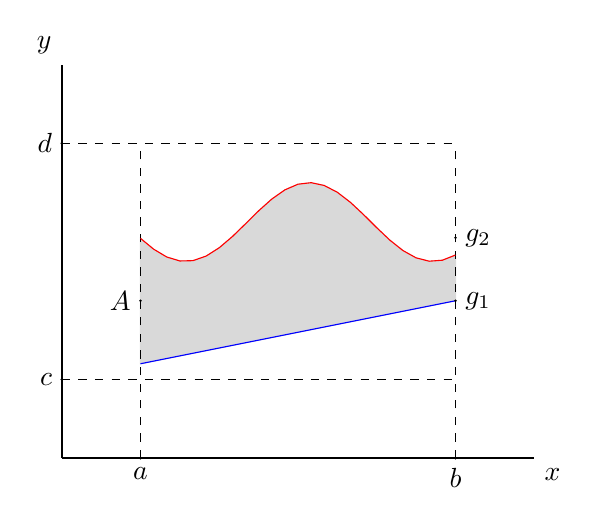
\begin{tikzpicture}
	\filldraw[gray!30] plot [domain=1:5] ({\x},{3 + (1/2)*cos(2*\x r)})
-- plot [domain=5:1] ({\x},{1+0.2*\x})
-- cycle;
		\draw[thick](0,0) -- (6,0) node[anchor=north west] {$x$};
		\draw[thick] (0,0) -- (0,5) node[anchor=south east] {$y$};
		\draw [dashed](0,1) -- (5,1);
		\draw [dashed](0,4) -- (5,4);
		\draw [dashed](1,0) -- (1,4);
		\draw [dashed](5,0) -- (5,4);
		
		
		\draw[domain=1:5,variable=\x,blue] plot ({\x},{1+0.2*\x});
		\draw[domain=1:5,variable=\x,red] plot ({\x},{3 + (1/2)*cos(2*\x r)});
		
		
		\fill (1,0) circle (0.5pt)node[anchor=north] {$a$};
		\fill (5,0) circle (0.5pt)node[anchor=north] {$b$};
		\fill (0,1) circle (0.5pt)node[anchor=east] {$c$};
		\fill (0,4) circle (0.5pt)node[anchor=east] {$d$};
		\fill (1,2) circle (0.5pt)node[anchor=east] {$A$};
		\fill (5,2) circle (0.5pt)node[anchor=west] {$g_1$};
		\fill (5,2.8) circle (0.5pt)node[anchor=west] {$g_2$};
	\end{tikzpicture}
	\end{center}
	\end{figura}
	Sean $\function{g_1,g_2}{[a,b]}{\R}$ continuas, tal que $g_1(x)\leq g_2(x)\ \forall x\in [a,b]$ y sea\\
	$A=\{(x,y)\in\R^2:x\in [a,b],g_1(x)\leq y\leq g_2(x) \}$. Calcular la integral de $\function{f}{A}{\R}$.\\
	$\integral{}{A}f(x,y)dxdy=\integral{}{[a,b]\times[c,d]}\overline{f}(x,y)dxdy=\integral{b}{a}\left(\integral{d}{c}\overline{f}(x,y)dy\right)dx$ \\
	Tenemos que $\integral{d}{c}\overline{f}(x_0,y)dy=\integral{g_1(x_0)}{c}\equals{\overline{f}(x_0,y)dy}{0}+\integral{g_2(x_0)}{g_1(x_0)}\overline{f}(x_0,y)dy+\integral{d}{g_2(x_0)}\equals{\overline{f}(x_0,y)dy}{0}=\\
=\integral{g_2(x_0)}{g_1(x_0)}f(x_0,y)dy$\\
$\implies \integral{}{A}f(x,y)dxdy=\integral{b}{a}\left(\integral{g_2(x)}{g_1(x)}f(x,y)dy\right)dx$
	\end{ejem}
	\newpage
	\begin{ejem} \ 
	\begin{figura}\ 
	\begin{center}
	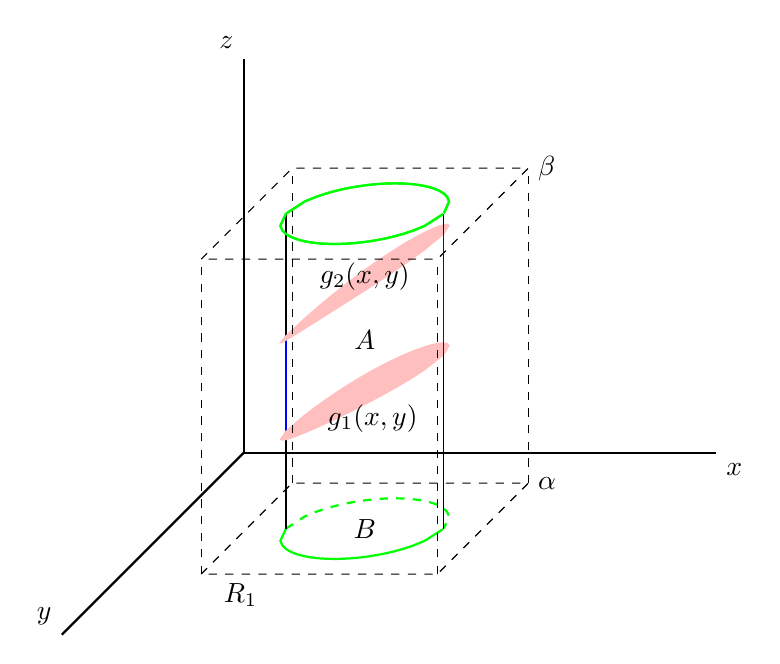
\begin{tikzpicture}
	\draw[thick](0,0,0) -- (6,0,0) node[anchor=north west] {$x$};
	\draw[thick] (0,0,0) -- (0,5,0) node[anchor=south east] {$z$};
	\draw[thick] (0,0,0) -- (0,0,6) node[anchor=south east] {$y$};
	\draw[domain=1.5:3.5,green,thick] plot (\x,0,{(1-(\x-2.5)^2)^(1/2)+2.5});
	\draw[domain=1.5:3.5,dashed,green, thick] plot (\x,0,{-(1-(\x-2.5)^2)^(1/2)+2.5});
	\draw[domain=1.5:3.5,green,thick] plot (\x,4,{(1-(\x-2.5)^2)^(1/2)+2.5});
	\draw[domain=1.5:3.5,green, thick] plot (\x,4,{-(1-(\x-2.5)^2)^(1/2)+2.5});
	
	
	\draw (1.5,0,2.5) -- (1.5,4,2.5);
	\draw [blue](1.5,1.2,2.5) -- (1.5,2.4,2.5);
	
	\filldraw[domain=1.5:3.5,variable=\x,pink] plot (\x,{2*(\x)^(1/2)},{(1-(\x-2.5)^2)^(1/2)+2.5}) plot (\x,{2*(\x)^(1/2)},{-(1-(\x-2.5)^2)^(1/2)+2.5});
	\filldraw[domain=1.5:3.5,variable=\x,pink] plot (\x,{1.5*(\x)^(1/2)-0.6},{(1-(\x-2.5)^2)^(1/2)+2.5}) plot (\x,{1.5*(\x)^(1/2)-0.6},{-(1-(\x-2.5)^2)^(1/2)+2.5});
	
	\draw[dashed]  (1,0,4) -- (1,0,1) -- (4,0,1) -- (4,0,4) -- (1,0,4);
	\draw (1.5,0,4) node[anchor=north] {$R_1$};
	\draw[dashed]  (1,0,1) -- (1,4,1);
	\draw[dashed]  (4,0,1) -- (4,4,1);
	\draw[dashed]  (4,0,4) -- (4,4,4);
	\draw[dashed]  (1,0,4) -- (1,4,4);	
	\draw[dashed]  (1,4,4) -- (1,4,1) -- (4,4,1) -- (4,4,4) -- (1,4,4);
	\draw (3.5,0,2.5) -- (3.5,4,2.5);
	\draw[blue] (3.5,2.2,2.5) -- (3.5,3.8,2.5);
	
	\draw (2.5,3.2,2.5)node {$g_2(x,y)$};
	\draw (2.6,1.4,2.5)node {$g_1(x,y)$};
	\draw (2.5,0,2.5)node {$B$};
	\draw (2.5,2.4,2.5)node {$A$};
	\draw (4,0,1)node[anchor=west]{$\alpha$};
	\draw (4,4,1)node[anchor=west] {$\beta$};
	\draw[domain=1.5:3.5,green,thick] plot (\x,4,{(1-(\x-2.5)^2)^(1/2)+2.5});
	\draw[domain=1.5:3.5,green, thick] plot (\x,4,{-(1-(\x-2.5)^2)^(1/2)+2.5});
	
	\end{tikzpicture}
	\end{center}
	\end{figura}
	Sea $B\subset \R^2$, sean $\function{g_1,g_2}{B}{\R}$ cumpliendo $g_1\leq g_2$. Sea\\
	$A=\{(x,y,z)\in \R^3:(x,y)\in B,g_1(x,y)\leq z\leq g_2(x,y)\}$. Calcular la integral de $\function{f}{A}{\R}$.\\
	$\integral{}{A}f=\underset{R=R_1\times[\alpha,\beta]}{\integral{}{R}\overline{f}}\overset{\mathrm{T.\ Fubini}}= \integral{}{R_1}\left(\integral{\beta}{\alpha}\overline{f}(x,y,z)dz\right)dxdy=\\
	=\integral{}{B}\left(\integral{\beta}{\alpha}\overline{f}(x,y,z)dz\right)dxdy+\equals{\integral{}{R_1\setminus B}\left(\integral{\beta}{\alpha}\overline{f}(x,y,z)dz\right)dxdy}{0}=\\
	=\integral{}{B}\left(\integral{\beta}{\alpha}\overline{f}(x,y,z)dz\right)dxdy=\\
	=\integral{}{B}\left(
	\equals{\integral{g_1(x,y)}{\alpha}\overline{f}(x,y,z)dz}{0} +		
	\integral{g_2(x,y)}{g_1(x,y)}\overline{f}(x,y,z)dz +
	\equals{\integral{\beta}{\alpha}\overline{f}(x,y,z)dz}{0}\right)dxdy=\\
	=\boxed{\integral{}{B}\left(\integral{g_2(x,y)}{g_1(x,y)}\overline{f}(x,y,z)dz\right)dxdy}$
	\end{ejem}
	\newpage
	\begin{ejem} Volumen de revolución de la gráfica de una función $f$ al girarla sobre el eje $OX$.\\
	\begin{figura}\ \\
		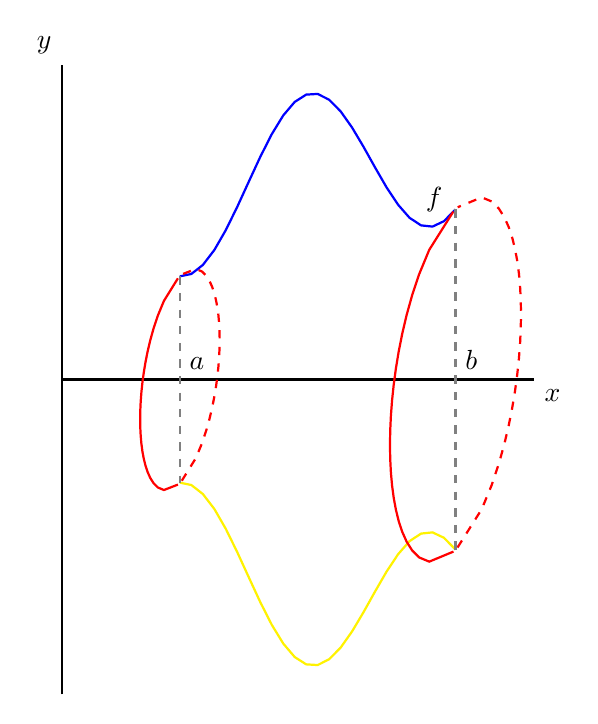
\begin{tikzpicture}
	\draw[thick](0,0,0) -- (6,0,0) node[anchor=north west] {$x$};
	\draw[thick] (0,-4,0) -- (0,4,0) node[anchor=south east] {$y$};	
	\draw[domain=1.5:5,blue,thick] plot (\x,{2+0.2*\x+cos(2*\x r)},0);
\draw[domain=1.5:5,yellow,thick] plot (\x,{-2-0.2*\x-cos(2*\x r)},0);	
	\draw[red,thick,variable=\y,domain=-1.31:1.31] plot (1.5,\y,{(1.72-(\y*\y))^(1/2)});
	\draw[dashed,red,thick,variable=\y,domain=-1.31:1.31] plot (1.5,\y,{-(1.72-(\y*\y))^(1/2)});

	\draw[red,thick,variable=\y,domain=-2.16:2.16] plot (5,\y,{(4.67-(\y*\y))^(1/2)});
	\draw[dashed,red,thick,variable=\y,domain=-2.16:2.16] plot (5,\y,{-(4.67-(\y*\y))^(1/2)});
	\draw[dashed,gray,thick] (1.5,1.31,0) -- (1.5,-1.31,0);
	\draw[dashed,gray,thick] (5,2.16,0) -- (5,-2.16,0);
	\draw (5,0,0) node[anchor=south west] {$b$};
	\draw (1.5,0,0) node[anchor=south west] {$a$};
	\draw (4.5,2,0) node[anchor=south west] {$f$};
	\end{tikzpicture}
	\end{figura}
	\ \\ Volumen$(V)=\integral{b}{a}$Área$(V_x)dx=\integral{b}{a}\pi f(x)^2dx=\pi\integral{b}{a}f(x)^2dx$
	\end{ejem}